% QMC in the VB Basis Chapter
%======================================================================
%======================================================================
\chapter{Quantum Monte Carlo in the Valence Bond Basis}

\comment{REFERENCES!!}

{\color{red} - VB QMC is a T=0, GS projection technique (redundant? Yes)}
\\
%======================================================================
%======================================================================
\section{The Valence Bond Basis}
%--------------------------------------------------------------------------------------------------------------------------
%What is a VB and how can it be represented?\\
%Representing multiple VBs\\
%VB basis properties\\

{\color{red} The valence bond basis, like the $S^Z$ basis, can be used to represent spin states.}
%--------------------------------------------------------------------------------------------------------------------------
\subsection{The Spin 1/2 Singlet State}
%--------------------------------------------------------------------------------------------------------------------------

Typically the states of spin 1/2 particles are represented in the $S^Z$ basis.  
\notsay{ 
Applying the $S^Z$ operator to its eigenstates yields either $+1/2$ or $-1/2$ 
corresponding to the spin up and spin down eigenstates respectively.
\begin{equation}
 	  S^z\lvert \uparrow \rangle = +\frac{1}{2} \lvert \uparrow \rangle
 	 \:\:\:    \:\:\:    \:\:\:    \:\:\:    \:\:\:    \:\:\: 
 	  S^z\lvert \downarrow \rangle = -\frac{1}{2} \lvert \downarrow \rangle
	   \label{SZ}
\end{equation}
}
A singlet state refers to a spin state of a particle or group of particles with vanishing total spin angular momentum.
%other states are not eigenstates of S^2
For two spin 1/2 particles there is exactly one singlet state, represented in the $S^Z$ basis as

\begin{equation}
  \frac{1}{\sqrt{2}}\left( \lvert \uparrow_a \downarrow_b \rangle - \lvert \downarrow_a \uparrow_b \rangle \right).
   \label{singlet}
\end{equation}
We can see this explicitly by finding the eigenstates of the $S^2$ operator for 
two spin 1/2 particles.  We begin by expressing the $S^2$ operator in terms of its different
spin components:
\begin{eqnarray}
S^2 &=& (S^x)^2 + (S^y)^2 + (S^z)^2 \\
(S_a + S_b)^2 &=& (S^x_a+S^x_b)^2 + (S^y_a+S^y_b)^2 + (S^z_a+S^z_b)^2 \nonumber \\
			&=&(S^x\otimes I+I \otimes S^x)^2 + 
			(S^y\otimes I+I\otimes S^y)^2 + (S^z\otimes I+I\otimes S^z)^2
			\label{s2}
\end{eqnarray}
where $I$ is the 2x2 identity matrix.  In Eq.~\eqref{s2} the operators are single spin operators.
Switching to matrix notation now, we have
\begin{eqnarray}
(S_a + S_b)^2 &=& 
\left(
	\frac{1}{2}
	\left[  \begin{array}{cc}
	0 & 1\\
	1 & 0\\
 	\end{array} \right] \otimes 
 	\left[  \begin{array}{cc}
	1 & 0\\
	0 & 1\\
	 \end{array} \right] 
	 +
	 	\frac{1}{2}
	\left[  \begin{array}{cc}
	1 & 0\\
	0 & 1\\
 	\end{array} \right] \otimes \nonumber
 	\left[  \begin{array}{cc}
	0 & 1\\
	1 & 0\\
	 \end{array} \right] 
	 \right)^2\\
	 &&+
	 \left(
	\frac{1}{2}
	\left[  \begin{array}{cc}
	0 & -i\\
	i & 0\\
 	\end{array} \right] \otimes 
 	\left[  \begin{array}{cc}
	1 & 0\\
	0 & 1\\
	 \end{array} \right] 
	 +
	 	\frac{1}{2}
	\left[  \begin{array}{cc}
	1 & 0\\
	0 & 1\\
 	\end{array} \right] \otimes 
 	\left[  \begin{array}{cc}
	0 & -i\\
	i & 0\\
	 \end{array} \right] 
	 \right)^2\\
	 &&+
	 \left(
	\frac{1}{2}
	\left[  \begin{array}{cc}
	1 & 0\\
	0 & -1\\
 	\end{array} \right] \otimes 
 	\left[  \begin{array}{cc}
	1 & 0\\
	0 & 1\\
	 \end{array} \right] 
	 +
	 	\frac{1}{2}
	\left[  \begin{array}{cc}
	1 & 0\\
	0 & 1\\
 	\end{array} \right] \otimes 
 	\left[  \begin{array}{cc}
	1 & 0\\
	0 & -1\\
	 \end{array} \right] 
	 \right)^2\nonumber \\
	 &=& \left[  \begin{array}{cccc}
	2 & 0 & 0 & 0\\
	0 & 1 & 1 & 0\\
	0 & 1 & 1 & 0\\
	0 & 0 & 0 & 2\\
	 \end{array} \right]
	 \label{diagon}
\end{eqnarray}
where the eigenvalues and eigenvectors are:
\begin{eqnarray}
\lambda_1 = 2,  &\mathbf{v}_1 = \left[ \begin{array}{cccc}1&0&0&0\end{array}  \right] ^\top
	 &= \lvert \uparrow \uparrow \rangle \nonumber\\
	 \lambda_2 = 2,  &\mathbf{v}_2 = \left[ \begin{array}{cccc}0&0&0&1\end{array}  \right] ^\top
	 &= \lvert \downarrow \downarrow \rangle \nonumber\\
	 \lambda_3 = 2,  &\;\;\;\;\,\mathbf{v}_3 =\tfrac{1}{\sqrt{2}}
	  \left[ \begin{array}{cccc}0&1&1&0\end{array}  \right]^\top
	 &= \tfrac{1}{\sqrt{2}} \big(
	 \lvert \uparrow \downarrow \rangle + \lvert \downarrow \uparrow \rangle \big) \nonumber\\
	  \lambda_4 = 0,  &\;\;\;\;\;\;\;\;\mathbf{v}_4 =\tfrac{1}{\sqrt{2}}
	  \left[ \begin{array}{cccc}0&1&-1&0\end{array}  \right]^\top
	 &= \tfrac{1}{\sqrt{2}} \big(
	 \lvert \uparrow \downarrow \rangle - \lvert \downarrow \uparrow \rangle \big).
\end{eqnarray}
There is only one state with total spin equal to zero.  The other three states have total spin 1. 
(If $\lvert \psi\rangle$ is a total spin eigenstate then 
$S^2\lvert\psi\rangle = s(s+1)\lvert\psi\rangle$, where $s$ is the total spin.)
%--------------------------------------------------------------------------------------------------------------------------
\subsubsection{Aside: Equivalence of the valence bond and the singlet state}
%--------------------------------------------------------------------------------------------------------------------------
{\it{A bond between two atoms created by sharing valence electrons in the outer orbitals is called a valence bond, or a covalent bond \cite{Slater1931,Pauling1933}.
Since electrons are fermionic (have half integer spin) their total
wave function must be antisymmetric (an exchange of the identical particles in the wave function
gives a factor of -1, i.e. $\Psi(1,2) = -\Psi(2,1)$).
The total wave function is a product of the spatial and spin wave functions, so one of those wave functions must be antisymmetric and the other symmetric (an exchange of particles yields the same wave function, i.e. $\Psi(1,2) = \Psi(2,1)$).
As part of the same valence bond, two electrons will have a symmetric spatial wave function {\color{red} true?}, so their spin state must be antisymmetric.  For two spin 1/2 particles the only antisymmetric spin state is the singlet state.  
Hence, in the case of two spin 1/2 particles, a valence bond is equivalent to the spin 1/2 singlet state from equation \eqref{singlet}.}}
%--------------------------------------------------------------------------------------------------------------------------
We represent these valence bonds, or singlet states, in three ways: 
\begin{itemize}
\item{in the $S^z$ basis using up spins and down spins, 
i.e. $\tfrac{1}{\sqrt{2}}( \lvert \uparrow_a \downarrow_b \rangle - \lvert \downarrow_a \uparrow_b \rangle)$,}
\item{ as a list of the bonded sites, i.e. $\lvert(a,b)\rangle$,}
\item{
or pictorially as a bond joining two sites. (See Figure~\ref{bond}.)}
\end{itemize}

\begin{figure} { 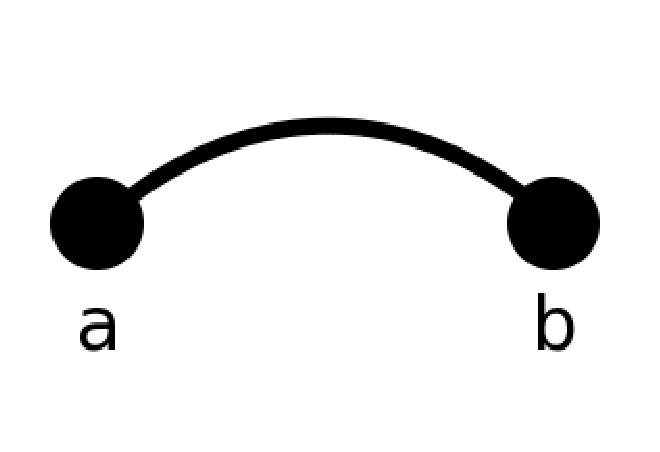
\includegraphics [width=2in]
{./figures/made/bond.eps}
\centering
 \caption[A \change{diagrammatic} representation of a valence bond]{
 A pictorial representation of a valence bond joining sites a and b.}
 }
\label{bond}
\end{figure}

{\color{red} anything about it being maximally entangled?}

%--------------------------------------------------------------------------------------------------------------------------
\subsection{Basis Properties}
%--------------------------------------------------------------------------------------------------------------------------
A collection of sites on a lattice can be paired into a valence bonds such that each site
belongs to exactly one bond (see in Figure~\ref{covering}).  
We call this a valence bond covering, and it is most conveniently represented as a list of 
sites that are paired in valence bonds:
\begin{equation}
	\ket{V} = \ket{(i_1,j_1)(i_2,j_2)\cdots(i_N,j_N)},
\end{equation}
where bonds go from sites $i$ to $j$ for a lattice with $2N$ sites.  
\notsay{Changing the order of the bonds in this list will not change the state, but reversing the order of an
$i$, $j$ pair may.}

\begin{figure} { 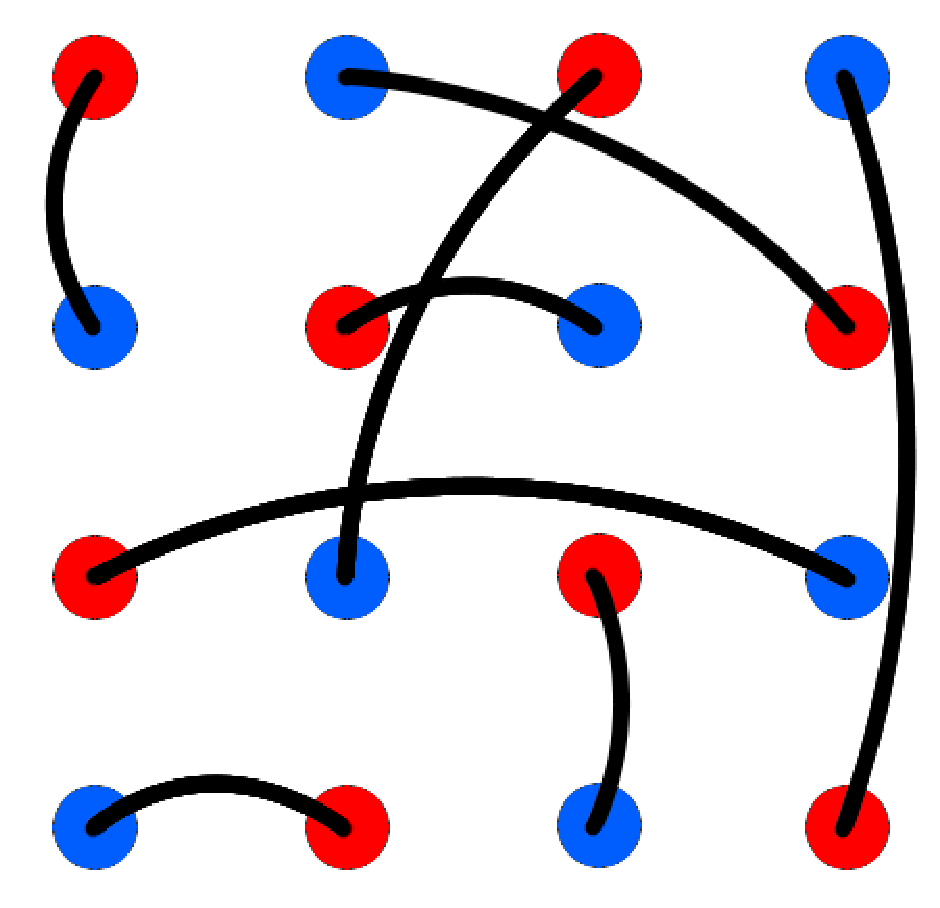
\includegraphics [width=3in]
{./figures/made/covering.eps}
\centering
 \caption[An example of a valence bond covering]{
 \comment{Maybe redo this figure.} An example of a valence bond covering.
 }
 }
\label{covering}
\end{figure}
 
A basis of valence bond coverings can be used to represent an arbitrary singlet state
for an even number of spins, but in general that representation is not unique.

The number of possible singlet states for a given number of spin 1/2 sites can be enumerated
using the rule for the addition of angular momentum for each added spin,
\begin{equation}
	S\otimes \tfrac{1}{2}  = \left(S-\tfrac{1}{2}\right)\oplus\left(S+\tfrac{1}{2}\right),
\end{equation}
where S is the $(2S+1)$-degenerate state of spin $S$ \cite{Beach2006}.
\begin{eqnarray}
	\tfrac{1}{2} \otimes \tfrac{1}{2}  &=& 0 \oplus 1\nonumber \\ 
	\tfrac{1}{2} \otimes \tfrac{1}{2}  \otimes \tfrac{1}{2} &=& 
	\tfrac{1}{2} \oplus  \tfrac{1}{2} \oplus  \tfrac{3}{2} \nonumber \\
	\tfrac{1}{2} \otimes \tfrac{1}{2}  \otimes \tfrac{1}{2} \otimes \tfrac{1}{2} &=& 
	0 \oplus 0 \oplus 1 \oplus 1 \oplus 1 \oplus 2 \nonumber \\
	\tfrac{1}{2} \otimes \tfrac{1}{2}  \otimes \tfrac{1}{2}  \otimes \tfrac{1}{2}  \otimes \tfrac{1}{2}&=& 
	\tfrac{1}{2} \oplus \tfrac{1}{2} \oplus \tfrac{1}{2} \oplus \tfrac{1}{2} \oplus \tfrac{1}{2} \oplus  
	\tfrac{3}{2} \oplus \tfrac{3}{2} \oplus \tfrac{3}{2} \oplus \tfrac{3}{2} \oplus
	  \tfrac{5}{2} \nonumber \\
	\tfrac{1}{2} \otimes \tfrac{1}{2}  \otimes \tfrac{1}{2} \otimes \tfrac{1}{2} \otimes \tfrac{1}{2}
	\otimes \tfrac{1}{2} &=& 
	\underbrace{0 \oplus\cdots \oplus 0}_{5 \rm{\; times}} \oplus 
	\underbrace{1 \oplus \cdots \oplus 1}_{9 \rm{\; times}} \oplus 
	\underbrace{2 \oplus \cdots \oplus 2}_{5 \rm{\; times}} 
	\oplus 3 \nonumber
\end{eqnarray}
For and even number of spins, 2N, the number of singlet states is given by 
\begin{equation}
	C_{\rm{sing}}^N = \frac{1}{N+1}\binom{2N}{N}\ = \frac{(2N)!}{N!(N+1)!},
\end{equation}  
and each of these singlet states is linearly independent of the others.
{\color{red} Can I figure out what the states actually look like?  Why is it 1/(n+1)(2n choose n)?}
In contrast, the number of possible valence bond states is given by
\begin{equation}
	C_{\rm{VB}}^N =
	\frac{(2N)!}{2^NN!},
\end{equation}
since we choose sites at random ($2N!$ ways to choose them) pairing them, but the order 
in which each member of the bond is chosen does not matter (divide by 2 for every bond), 
nor does the order in which the $N$ bonds are chosen (divide by $N!$).
For $N>1$ there are more valence bond coverings than singlet states, the excess increasing 
drastically by increasing $N$.  

The valence bond states are not orthogonal to each other, in fact every valence bond covering
has some overlap with every other covering.
Because of this overcompleteness we can eliminate some of the valence bond states and still
represent any singlet state.  
In fact, this can be seen for a four-site system by again diagonalizing the $S^2$ matrix.
This time we will only look at the $S^z=0$ sector, since all the singlet states will be found there.
With the same method used to get \eqref{diagon}, we find:
\begin{eqnarray}
S^2_{\text{reduced}} =\left[
\begin{array}{cccccc}
2&1&1&1&1&0\\
1&2&1&1&0&1\\
1&1&2&0&1&1\\
1&1&0&2&1&1\\
1&0&1&1&2&1\\
0&1&1&1&1&2\\
\end{array} \right] 
\begin{array}{cl}
\lambda_1=6,&\mathbf{v_1} =\left[\begin{array}{cccccc} 1&1&1&1&1&1\end{array} \right]\\
\lambda_2=2,&\mathbf{v_2} =\left[\begin{array}{cccccc} 1&0&0&0&0&-1\end{array} \right]\\
\lambda_3=2,&\mathbf{v_3} =\left[\begin{array}{cccccc} 0&1&-3&3&-1&0\end{array} \right]\\
\lambda_4=2,&\mathbf{v_4} =\left[\begin{array}{cccccc} 0&3&1&-1&-3&0\end{array} \right]\\
\lambda_5=0,&\mathbf{v_5} =\left[\begin{array}{cccccc} 0&1&-1&-1&1&0\end{array} \right]\\
\lambda_6=0,&\mathbf{v_6} =\left[\begin{array}{cccccc} 1&-1&0&0&-1&1\end{array} \right]\\
\end{array} 
\end{eqnarray}
where $\mathbf{v_5}$ and $\mathbf{v_6}$ are the (so far unnormalized) singlet states.
Note that there are only two linearly independent singlet states, while there are three valence bond states
for a four-site system.
Also interesting is that the singlet states are composed of two-site valence bonds. 
Expressing $\mathbf{v_5}$ and $\mathbf{v_6}$ in the spin and valence bond bases we get
\begin{eqnarray}
\mathbf{v_5} &=&\frac{1}{2}\bigg(\lvert \dw \up \dw \up \rangle - \lvert \dw \up \up \dw \rangle
			- \lvert \up \dw \dw \up \rangle + \lvert \up \dw \up \dw \rangle \bigg) 
			= \lvert(a,b)(c,d)\rangle\\
\mathbf{v_6} &=&\frac{1}{2}\bigg(\lvert \dw \dw \up \up \rangle - \lvert \dw \up \up \dw \rangle
			- \lvert \up \dw \dw \up \rangle + \lvert \up \up \dw \dw \rangle \bigg)
			= \lvert(a,d)(c,b)\rangle
\end{eqnarray}
{\color{red} is there a way to get little vb diagrams in there? - note: also made up of vbs.
Talk about how we can express the 3rd VB config in terms of the other two.}


It is convenient to define two sublattices, A and B, on a bipartite lattice, such that sites on 
sublattice A are neighbored only by sublattice B sites and vice versa. (See figure~\ref{covering}
where the red sites belong to sublattice A and the blue sites belong to sublattice B.  Note that there are only A-B sublattice bonds present.)
We can choose the valence bond coverings containing only bonds going from sublattice A
to B.  (I say ``from A to B" because valence bonds are directional; the ordering of the
sites matters, and reversing the order gives a factor of -1.)
This restriction eliminates some, though not all, of the overcompleteness of the states.
The, now reduced, number of valence bond states is simply $C_{\rm{AB}}^N = N!$ for a system of $2N$ spins.

One way to see the linear dependence of these valence bond states would be to again diagonalize
the $S^2$ matrix, for a six-site system this time (in which there are $3!=6$ A-B sublattice
valence bond states, but only $6!/(3!4!) = 5$ singlet states).
This, however, would require us to diagonalize a 64x64 matrix, or a 20x20 matrix if we only look at
the $S^z=0$ sector.


{\color{red} Perhaps, show how even with the AB sublattice coverings only, it's still overcomplete.
Though I do this using the *overlap* matrix, which I need to compute the overlap for... and I haven't
said how the calculate the overlap.  Where is that going to go, btw?}


{\color{red} graph comparing the functions}
{\color{red} maybe show some of my awesome matrix calculations? \\ 
the lack of linear independence for N=3.}

{\color{red}
- then actually go over the properties if they haven't already been mentioned.

- VB basis can be used to represent any singlet state\\
- spans the spin 0 sector\\
***- singlets have a lower energy that the classical N\'eel state\\
- show how we represent VB's and VB coverings
}

{\color{red} Fazekas and Anderson said it's a good choice for the heis s=1/2 antiferro GS
because it has total spin zero, and lower energy than the N\'eel state.  check if this is true.}

{\color{red} Thing from Anderson 1973 about energy per NN VB vs energy per 2 antiparallel sites,
but with math and stuff this time.}

\subsection{The Inner Product}

{\color{red} show pictures and stuff.  Show mathematically how the VB overlap is calculated,
representing the VBs in the Sz basis.}


%--------------------------------------------------------------------------------------------------------------------------
\section{Ground State Projection} \label{gsp}
%--------------------------------------------------------------------------------------------------------------------------
{\color{red} maybe somewhere in this section do the whole "we can represent any singlet states in
terms of valence bond states *EQUATION*, though that representation is not unique (even with just
the AB sublattice VBs) for more than 4 sites.  How*ever* we can always represent a state uniquely 
in terms of it's energy eigenstates..."}

Quantum Monte Carlo in the valence bond basis is a ground state projection technique, 
which means we start with a trial wave function apply high powers of the Hamiltonian until 
we are left with the zero temperature ground state of the system. 
\notsay{
Though, being that it is a
Monte Carlo technique, we are not actually left with the wave function, but we sample terms in
the ground state wave function and we can then sample observable properties
 according to the statistics of the 
ground state wave function.\\
}
{\color{red} explain GS projection real good now.}

Though valence bond states are not necessarily represented uniquely, an arbitrary state can 
always be represented as a unique combination of the energy eigenstates of a Hamiltonian,
\begin{equation}
\lvert \psi \rangle = \sum_n c_n \lvert n \rangle,
\label{state}
\end{equation}
where $\lvert n \rangle$ is the $n^{\rm{th}}$ energy eigenstate of a Hamiltonian and the 
$c_n$\!'s are
the unique coefficients.

If we apply the Hamiltonian to the state in Eq.~(\ref{state}) we are left with
\begin{equation}
\mathcal{H}\lvert \psi \rangle = \sum_n c_n \mathcal{H} \lvert n \rangle =
 		\sum_n c_n E_n \lvert n \rangle = 
		c_0 E_0 \lvert 0 \rangle + c_1 E_1 \lvert 1 \rangle +
		c_2 E_2 \lvert 2 \rangle + \cdots,
\end{equation}
where $E_n$ is the $n^{\rm{th}}$ energy eigenvalue of the Hamiltonian, $\mathcal{H}$.
We can then take out a factor of $E_0$ to get
\begin{equation}
\mathcal{H}\lvert \psi \rangle =
		E_0 \left(c_0 \lvert 0 \rangle + c_1 \frac{E_1}{E_0} \lvert 1 \rangle +
		c_2\frac{ E_2}{E_0} \lvert 2 \rangle + \cdots \right).
\end{equation}

If $E_0$ is the energy largest in magnitude, then all the coefficients
of the excited states are fractions less (in magnitude) than 1.  
In that case, if we apply the Hamiltonian a large number of times, denoted by m, all terms excluding
the ground state term will vanish.
\begin{equation}
\mathcal{H}^m\lvert \psi \rangle =
		E_0^m \left(c_0 \lvert 0 \rangle + 
		c_1 \left(\frac{E_1}{E_0}\right)^m \lvert 1 \rangle +
		c_2\left(\frac{ E_2}{E_0}\right)^m \lvert 2 \rangle + \cdots \right)
		\approx E_0^m c_0 \lvert 0 \rangle
\end{equation}

{\color{red} Check the sign for this part.}
If the ground state energy is not the largest in magnitude, as is the case with the Heisenberg
model, we can manipulate the Hamiltonian slightly by adding or subtracting an
appropriately chosen constant term, $x$, in which case we will have
\begin{equation}
(x-\mathcal{H)}^m\lvert \psi \rangle =
		(E_0-x)^m \left(c_0 \lvert 0 \rangle + 
		c_1 \left(\frac{E_1-x}{E_0-x}\right)^m \lvert 1 \rangle  + \cdots \right)
		\approx (E_0-x)^m c_0 \lvert 0 \rangle.
\end{equation}

{\color{red} Comments to totally conclude up this section.}


%--------------------------------------------------------------------------------------------------------------------------
\section{The Hamiltonian and Bond Operators}
%--------------------------------------------------------------------------------------------------------------------------
Throughout this thesis we will be looking at the Heisenberg model in one and two dimensions,
and so the Hamiltonian used will be the isotropic, antiferromagnetic Heisenberg 
Hamiltonian:
\begin{equation}
\mathcal{H}_{\rm{Heis}}=J\sum_{\langle i,j \rangle} \mathbf{S}_i\cdot \mathbf{S}_j
= J\sum_{\langle i,j \rangle}
	\left( S_i^z S_j^z + \tfrac{1}{2}\left[ S_i^+ S_j^- + S_i^- S_j^+ \right]\right),
\end{equation}
where the coupling constant $J$ is always positive, and $\sum_{\langle i,j \rangle}$ 
represents a sum over all nearest-neighbor pairs of sites.  
\notsay{
If we apply this Hamiltonian to states in the $S^z$ basis, 
the first term will assign lower energy to pairs of sites with antiparallel spins,
while the remainder of the Hamiltonian will act to flip pairs of spins that are already 
antiparallel or annihilate states with parallel spins. 
}

We slightly modify the Hamiltonian for use in the ground state projection scheme:

\begin{equation}
\mathcal{H}= \left(\mathcal{H}_{\rm{Heis}} - \tfrac{1}{4} \right)= \sum_{\langle i,j \rangle} 
	\left(\mathbf{S}_i\cdot \mathbf{S}_j - \tfrac{1}{4}\right)
	= - \sum_{\langle i,j \rangle} H_{ij}.
\end{equation}
Here the coupling constant $J$ is set to 1, and rewrite the Hamiltonian in terms of a list of
\it{bond operators}, \rm $H_{ij}$, where 
$H_{ij}=-\left(\mathbf{S}_i\cdot \mathbf{S}_j - \tfrac{1}{4}\right)$.

The effect of these bond operators acting on a valence bond basis state is 
surprisingly simple.  If a bond operator acts on two sites already joined by a valence
bond, it acts as the identity and does not changed the state.  If the two sites acted upon are 
not joined in a valence bond, the operator joins those two sites, and as a byproduct the 
two sites that were once joined to those sites form a valence bond themselves.
This is depicted in {\color{red} picture of VBs and bond ops acting on them and stuff.}
It can also be shown mathematically, but first let's examine the effect of bond operators
on a general spin 1/2 state.

We can rewrite the dot product of spin operators:
\begin{eqnarray}
\mathbf{S}_i\cdot \mathbf{S}_j = \tfrac{1}{2}\left[ \left(S_i + S_j\right)^2 -S_i^2-S_i^2 \right],
\end{eqnarray}
and since we are dealing with spin 1/2 particles, applying the $S^2$ operators to any state will
give 
\begin{equation}
S^2\lvert \psi\rangle = s(s+1)\lvert \psi \rangle = \tfrac{1}{2}(\tfrac{1}{2} + 1)\lvert \psi \rangle
	= \tfrac{3}{4}\lvert\psi\rangle
\end{equation}
for an arbitrary spin 1/2 state, $\lvert \psi\rangle$.  However, the $\left(S_i + S_j\right)^2$ 
operator has two different eigenvalues, or it could change the state
if the initial state is not one of the four total spin eigenstates.

Acting on an eigenstate of the total spin operator for two spins with a bond operator yields:
\begin{equation}
H_{ij}\lvert \psi \rangle = \begin{cases}
	-\left(\tfrac{1}{2} \left[(0) - \tfrac{3}{4} - \tfrac{3}{4}\right] -\tfrac{1}{4}\right)\lvert\psi\rangle 
	= \lvert\psi\rangle \text{ for total spin 0}\\
	 -\left(\tfrac{1}{2} \left[(2) - \tfrac{3}{4}- \tfrac{3}{4}\right]-\tfrac{1}{4}\right)\lvert\psi\rangle
	 = 0 \text{ \;\;\;for total spin 1}
	 \end{cases}
	 \label{bop}
\end{equation}
If we want to use the bond operators on valence bond basis states Eq.~(\ref{bop}) tells
us what happens when sites $i$ and $j$ are already joined in a valence bond, but we still
need to look at the case in which the sites are initially part of two different valence bonds.
For four sites $a$, $b$, $c$, and $d$, with sites a and c on sublattice A 
and the other on sublattice B,
apply the operator $H_{cb}$
\begin{eqnarray}
H_{cb}\lvert(a,b)(c,d)\rangle &=& H_{cb}
	\tfrac{1}{\sqrt{2}} \big( 
	\lvert \uparrow_a \downarrow_b \rangle - \lvert \downarrow_a \uparrow_b \rangle 
	\big) 
	\tfrac{1}{\sqrt{2}} \big( 
	\lvert \uparrow_c \downarrow_d \rangle - \lvert \downarrow_c \uparrow_d \rangle 
	\big) \nonumber \\ 
	&=&
	  \tfrac{1}{2} H_{cb} \big(
	   \lvert\uparrow_a \downarrow_d\rangle \lvert \uparrow_c \downarrow_b \rangle
	   - \lvert \uparrow_a \uparrow_d \rangle \lvert \downarrow_c \downarrow_b \rangle
	   - \lvert \downarrow_a \downarrow_d \rangle \lvert \uparrow_c \uparrow_b \rangle
	   + \lvert \downarrow_a \uparrow_d \rangle \lvert \downarrow_c \uparrow_b \rangle
	   \big) \nonumber
\end{eqnarray}
At this point it is convenient to represent the spin states involving sites $b$ and $c$
in terms of eigenvalues of singlet and triplet states.
\begin{eqnarray}
H_{cb}\lvert(a,b)(c,d)\rangle &=&
	     \tfrac{1}{2} H_{cb} \left( \lvert\uparrow_a \downarrow_d \rangle 
	     \tfrac{1}{ \sqrt{2}} \left[ 
	     	\tfrac{1}{ \sqrt{2}} \big(
	     	\lvert \uparrow_c \downarrow_b \rangle - \lvert \downarrow_c \uparrow_b \rangle 
	     \big) + 
	     \tfrac{1}{ \sqrt{2}} \big(
	     \lvert \uparrow_c \downarrow_b \rangle + \lvert \downarrow_c \uparrow_b \rangle 
	     \big)
	     \right]
	     \right) \nonumber \\
	     &&
	     -   \tfrac{1}{2} H_{cb}
	     \Big(\lvert \uparrow_a \uparrow_d \rangle \lvert \downarrow_c \downarrow_b \rangle
	   + \lvert \downarrow_a \downarrow_d \rangle \lvert \uparrow_c \uparrow_b \rangle
	   \Big) \\
	   && - 	     \tfrac{1}{2} H_{cb} \left( \lvert\downarrow_a \uparrow_d \rangle 
	     \tfrac{1}{ \sqrt{2}} \left[ 
	     	\tfrac{1}{ \sqrt{2}} \big(
	     	\lvert \uparrow_c \downarrow_b \rangle - \lvert \downarrow_c \uparrow_b \rangle 
	     \big) -
	     \tfrac{1}{ \sqrt{2}} \big(
	     \lvert \uparrow_c \downarrow_b \rangle + \lvert \downarrow_c \uparrow_b \rangle 
	     \big)
	     \right]
	     \right) \nonumber
\end{eqnarray}
We are left with states for which we know the outcome of applying this bond operator.
The states with a nonzero total spin will vanish.
\begin{eqnarray}
H_{cb}\lvert(a,b)(c,d)\rangle &=&
	     \tfrac{1}{2}\left( \lvert\uparrow_a \downarrow_d \rangle 
	     \tfrac{1}{ \sqrt{2}} \left[ 
	     	\tfrac{1}{ \sqrt{2}} \big(
	     	\lvert \uparrow_c \downarrow_b \rangle - \lvert \downarrow_c \uparrow_b \rangle 
	     \big)
	     \right]
	     \right) \nonumber \\    
	   && \;\; \;\;\;\;\;\; \;\;\;\;\;
	    - 	     \tfrac{1}{2} \left( \lvert\downarrow_a \uparrow_d \rangle 
	     \tfrac{1}{ \sqrt{2}} \left[ 
	     	\tfrac{1}{ \sqrt{2}} \big(
	     	\lvert \uparrow_c \downarrow_b \rangle - \lvert \downarrow_c \uparrow_b \rangle 
	     \big)
	     \right]
	     \right) \nonumber \\
	     &=&  \tfrac{1}{2} \left[ \tfrac{1}{ \sqrt{2}} 
	     \big( \lvert\uparrow_a \downarrow_d \rangle - \lvert\downarrow_a \uparrow_d \rangle  
	     \big)\right]
	     \left[ \tfrac{1}{ \sqrt{2}} 
	     \big( \lvert\uparrow_c \downarrow_b \rangle - \lvert\downarrow_c \uparrow_b \rangle  
	     \big)\right] \\
	     &=& \tfrac{1}{2} \lvert(a,d)(c,b)\rangle \nonumber
\end{eqnarray}
As was asserted earlier, the operator acts to rearrange to bonds.
Also the state gains a factor of $\frac{1}{2}$.
{\color{red} And of course I need to write a bit more for this section... but about what?}


%--------------------------------------------------------------------------------------------------------------------------
\section{The Monte Carlo Algorithm}
%--------------------------------------------------------------------------------------------------------------------------
In section \ref{gsp} we saw that repeated application of the Hamiltonian to any initial state will
give us (\change{in the limit of a large power of the Hamiltonian}) a state proportional to the
ground state of the system.
However, computing this exactly would be \change{extremely computationally expensive}.
The Hamiltonian has $N_{nn}$ terms, one for each possible nearest-neighbor bond.  
Raising it to the even power $m$ would give us $N_{nn}^m$ terms each containing $m$ bond operators,
\begin{equation} \label{bopss}  
	\ham^m=\left(\sum_{r=1}^{N_{nn}}H_r\right)^m=
	\sum_{r_1=1}^{N_{nn}}\sum_{r_2=1}^{N_{nn}}\cdots \sum_{r_m=1}^{N_{nn}}
	\bigg( H_{r_1} H_{r_2} \cdots H_{r_m} \bigg) 
	=\sum_{r=1}^{N_{nn}^m} P_r,
\end{equation}
where $r$ goes over each of the possible nearest neighbor bonds.  
Applying $\ham^m$ to a trial state $\ket{V}$ gives us
\begin{equation} \label{hamapp}
	\ham^m \ket{V} = \sum_{r=1}^{N_{nn}^m} P_r \ket{V} = \sum_{r=1}^{N_{nn}^m} W(r)\ket{V(r)}
	= \sum_{r=1}^{N_{nn}^m} 2^{-m_r^{\text{off}}}\ket{V(P_r)},
\end{equation}
where $W(r)$ is the weight resulting from applying the $r^{\text{th}}$ term from \eqref{bopss} to 
the trial state, which is equivalent to the $1/2$ raised to the power of number of
 off-diagonal bond operators (bond operators
acting on sites that are not already joined by a valence bond) in $P_r$.

Instead of computing the full sum from \eqref{hamapp}, we stochastically sample terms
from the sum, with sampling proportional to their weight $W(r)$ in the sum.




\comment{actually put in the algorithms}

%--------------------------------------------------------------------------------------------------------------------------
\subsection{Single Projector}
%--------------------------------------------------------------------------------------------------------------------------
The single projector valence bond quantum Monte Carlo algorithm projects only one state \change{into}
the Heisenberg ground state.

\begin{enumerate}
\item \fbox{\parbox{410pt}{Choose or generate an initial valence bond state $\ket{V}$.}}
\item \fbox{\parbox{410pt}{Generate a list of m random bond operators $P_{\text{old}}$.}}
\item \fbox{\parbox{410pt}{Apply the list of bond operators to the initial state.  
		\begin{equation}
		P_{\text{old}}\ket{V}=W_{\text{old}}\ket{V_{\text{old}}} \nonumber
		\end{equation}
		}}
\item \fbox{\parbox{410pt}{Copy $P_{\text{old}}$ to $P_{\text{new}}$ 
		and randomly change a predetermined number, 
		$q$, of the bond operators 
		in $P_{\text{new}}$.}}
\item \fbox{\parbox{410pt}{Apply the new list of bond operators to the original initial state. 
		\begin{equation} P_{\text{new}}\ket{V}=W_{\text{new}}\ket{V_{\text{new}}}
		\nonumber
		\end{equation}
		}}
\item \fbox{\parbox{410pt}{
		Generate a random number $A \in [0,1)$.
		}}
\item \fbox{\parbox{410pt}{
		If $A < W_{\text{new}}/W_{\text{old}}$, relabel all ``new" quantities as ``old".
		}}
\item \fbox{\parbox{410pt}{		
		Take a measurement using the state $\ket{V_{\text{old}}}$. 		
		}}			
\item \fbox{\parbox{410pt}{
		Go to Step 4.	
		}}	
\end{enumerate}

%--------------------------------------------------------------------------------------------------------------------------
\subsubsection{Measurements}

\change{energy measurement}

\begin{equation}
	E_0 = \frac{\bra{R}\ham\ket{0}}{\bra{R}0\rangle} = 
	\frac{\bra{R}-\sum_{r=1}^{N_{nn}}H_r\ket{0}}{\bra{R}0\rangle} = 
	-\sum_{r=1}^{N_{nn}} \frac{\bra{R}H_r\ket{0}}{\bra{R}0\rangle}
\end{equation}
\change{If we choose the reference state $\ket{R}$ to be a classical N\'eel state, 
which has equal overlap with every valence bond state, 
we can further simplify this formula.}
\begin{equation}
	E_0 = -\sum_{r=1}^{N_{nn}} \frac{W(r)\bra{R}S_r\rangle}{\bra{R}0\rangle} =
	 -\sum_{r=1}^{N_{nn}} W(r) = -\left(\frac{n_{\text{off}}}{2} + n_{\text{diag}}\right),
\end{equation}
where $W(r)$ and $\ket{S_r}$ are the weight and the state gained by applying the $r^{\text{th}}$ bond operator to the ground state, $n_{\text{off}}$ is the number of off-diagonal bond operators 
in the Hamiltonian, and $n_{\text{diag}}$ is the number of diagonal bond operators in the Hamiltonian.

\comment{this isn't finished... i'm pretty sure}

\change{
- is there anything else we can measure? properties of the valence bonds.\\
- singlet-triplet gap? check sandvik's papers.
}
%--------------------------------------------------------------------------------------------------------------------------
\subsection{Double Projector}
%--------------------------------------------------------------------------------------------------------------------------
\change{
- similar to single projector, but two states are projected separately and the weights are different\\
- mention that single projector is not variational and double projector is\\
- can measure many other (non-energy) quantities 
}

\begin{enumerate}
\item \fbox{\parbox{410pt}{Choose or generate an initial valence bond state $\ket{V}$.}}
\item \fbox{\parbox{410pt}{Generate two lists of m random bond operators $L_{\text{old}}$
					and  $R_{\text{old}}$ .}}
\item \fbox{\parbox{410pt}{Apply the lists of bond operators to the initial state.  
		\begin{equation}
		\bra{V}L^\dagger_{\text{old}}=W^L_{\text{old}}\bra{V^L_{\text{old}}} \nonumber
		\;\;\;\;\;\;\;\;\;\;
		R_{\text{old}}\ket{V}=W^R_{\text{old}}\ket{V^R_{\text{old}}} 
		\end{equation}
		}}
\item \fbox{\parbox{410pt}{Copy $L_{\text{old}}$ to $L_{\text{new}}$ 
		and randomly change a predetermined number, 
		$q$, of the bond operators 
		in $L_{\text{new}}$.}}
\item \fbox{\parbox{410pt}{Apply the new left list of bond operators to the original initial state. 
		\begin{equation} 
			\bra{V}L^\dagger_{\text{new}}=W^L_{\text{new}}\bra{V^L_{\text{new}}} \nonumber			\end{equation}
		}}
\item \fbox{\parbox{410pt}{
		Generate a random number $A \in [0,1)$.	
		}}
\item \fbox{\parbox{410pt}{
		 If $A < W^L_{\text{new}}W^R_{\text{old}}\bra{V^L_{\text{new}}}V^R_{\text{old}}\rangle/
		 W^L_{\text{old}}W^R_{\text{old}}\bra{V^L_{\text{old}}}V^R_{\text{old}}\rangle$, 
		 relabel all ``new" left quantities as ``old".		
		 }}
\item \fbox{\parbox{410pt}{Randomly change a predetermined number, 
		$q$, of the bond operators 
		in $R_{\text{old}}$ and relabel it as $R_{\text{new}}$.}}
\item \fbox{\parbox{410pt}{Apply the new right list of bond operators to the original initial state. 
		\begin{equation} 
			R_{\text{new}}\ket{V}=W^R_{\text{new}}\ket{V^R_{\text{new}}}  \nonumber					\end{equation}
		}}
\item \fbox{\parbox{410pt}{
		Generate a random number $A \in [0,1)$.	
		}}
\item \fbox{\parbox{410pt}{
		 If $A < W^L_{\text{old}}W^R_{\text{new}}\bra{V^L_{\text{old}}}V^R_{\text{new}}\rangle/
		 W^L_{\text{old}}W^R_{\text{old}}\bra{V^L_{\text{old}}}V^R_{\text{old}}\rangle$, 
		 relabel all ``new" right quantities as ``old".		
		 }}
\item \fbox{\parbox{410pt}{		
		Take a measurement using the states $\bra{V^L_{\text{old}}}$ and
		$\ket{V^R_{\text{old}}}$. 			
		}}		
\item \fbox{\parbox{410pt}{
		Go to Step 4.	
		}}	
\end{enumerate}



%--------------------------------------------------------------------------------------------------------------------------
\subsection{Loop Moves}
%--------------------------------------------------------------------------------------------------------------------------
\comment{ do this section last... if there's time\\}
\change{
- sooooooooooooo fast \\
- drawbacks (can't change weight, like for renyi sampling thing)
}

